\documentclass[../main.tex]{subfiles}

\begin{document}

%% maybe mention CI pipeline on PR event?


%% 1) jenkins snapshot
%% compile, checks formatting, test
%% snapshot because publishes snapshot version to maven
%% 2 JARs: reqour-rest, reqour-adjuster

%% 2.1) reqour-adjuster-image job triggering Gitlab pipeline
%% build the image (using reqour-adjuster JAR)
%% push the image to quay.io

%% 2.2) reqour-image job triggering Gitlab pipeline
%% build the image (using reqour-erst JAR)
%% push the image to quay
%% apply (what's the correct word) the helm chart using that image
%% helm templating being used to define all the environemnts (devel, next-stable, stage, prod)

%% maybe note that snapshot triggers also sonarqube job?

Reqour deployment is done through CI/CD\footnote{Where \textit{D} stands for deployment, not delivery. Hence, the pipeline is fully automatized.} pipeline. The pipeline consists of 2 main parts: Jenkins and GitLab.

\section{Jenkins}
\subfile{./sections/jenkins}

\section{GitLab}
\subfile{./sections/gitlab}

Both Jenkins and GitLab parts are visualized (in less detail) in Figure \ref{fig:pipeline}.

\begin{figure}
  \begin{center}
    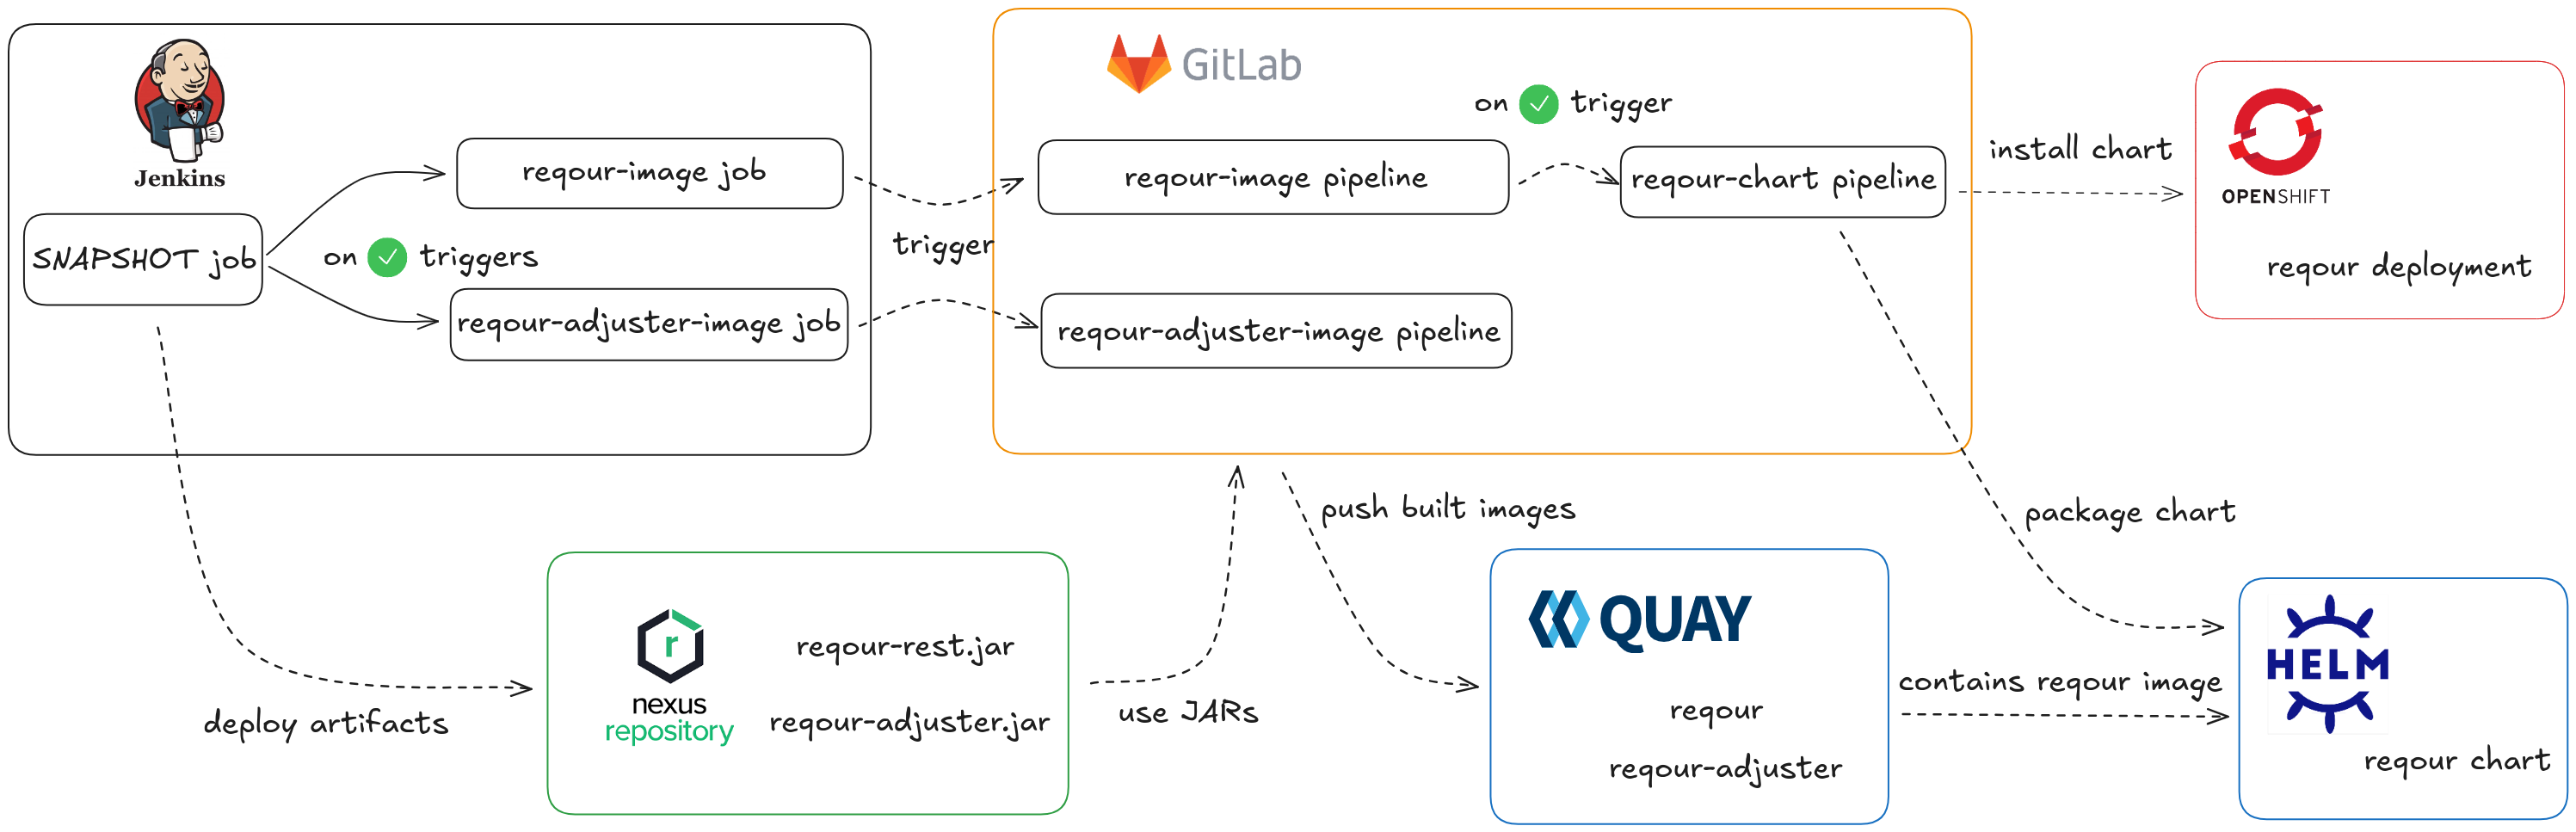
\includegraphics[width=\textwidth]{images/pipeline.png}
  \end{center}
  \caption{Pipeline}
  \label{fig:pipeline}
\end{figure}

\end{document}
